\chapter{利用法}
\label{chap:usage}
この章ではセンシングデータの利用法を具体的に提案する。\\
センシングデータといってもWeb上で取得できる物は全てデータとして扱うことが出来る。
例えば藤沢の気温データをWeb上から更新される度に取得することで気温のセンシングデータを作成できる。また、現在時刻やPCのファイル情報などユーザーのコンテキストも取得してデータにすることが出来る。
これらのデータを使えば条件指定の幅が広がり複雑なプログラムを簡単に書くことが出来る。

\section{ニュース購読}
現在時刻を取得することで簡単にアラーム機能を実装できる。指定の時間をすぎるとニュースを取得し、PCに喋らせているのが以下の例だ。Macのsayコマンドを使って特定のPCから音声を発信している。
(図\ref{fig:image10})では時間を取得するtimeオブジェクトが9時と21時にマッチした時にnewsにアクセスしている。
\begin{figure}[htbp]
  \begin{center}
    \fbox{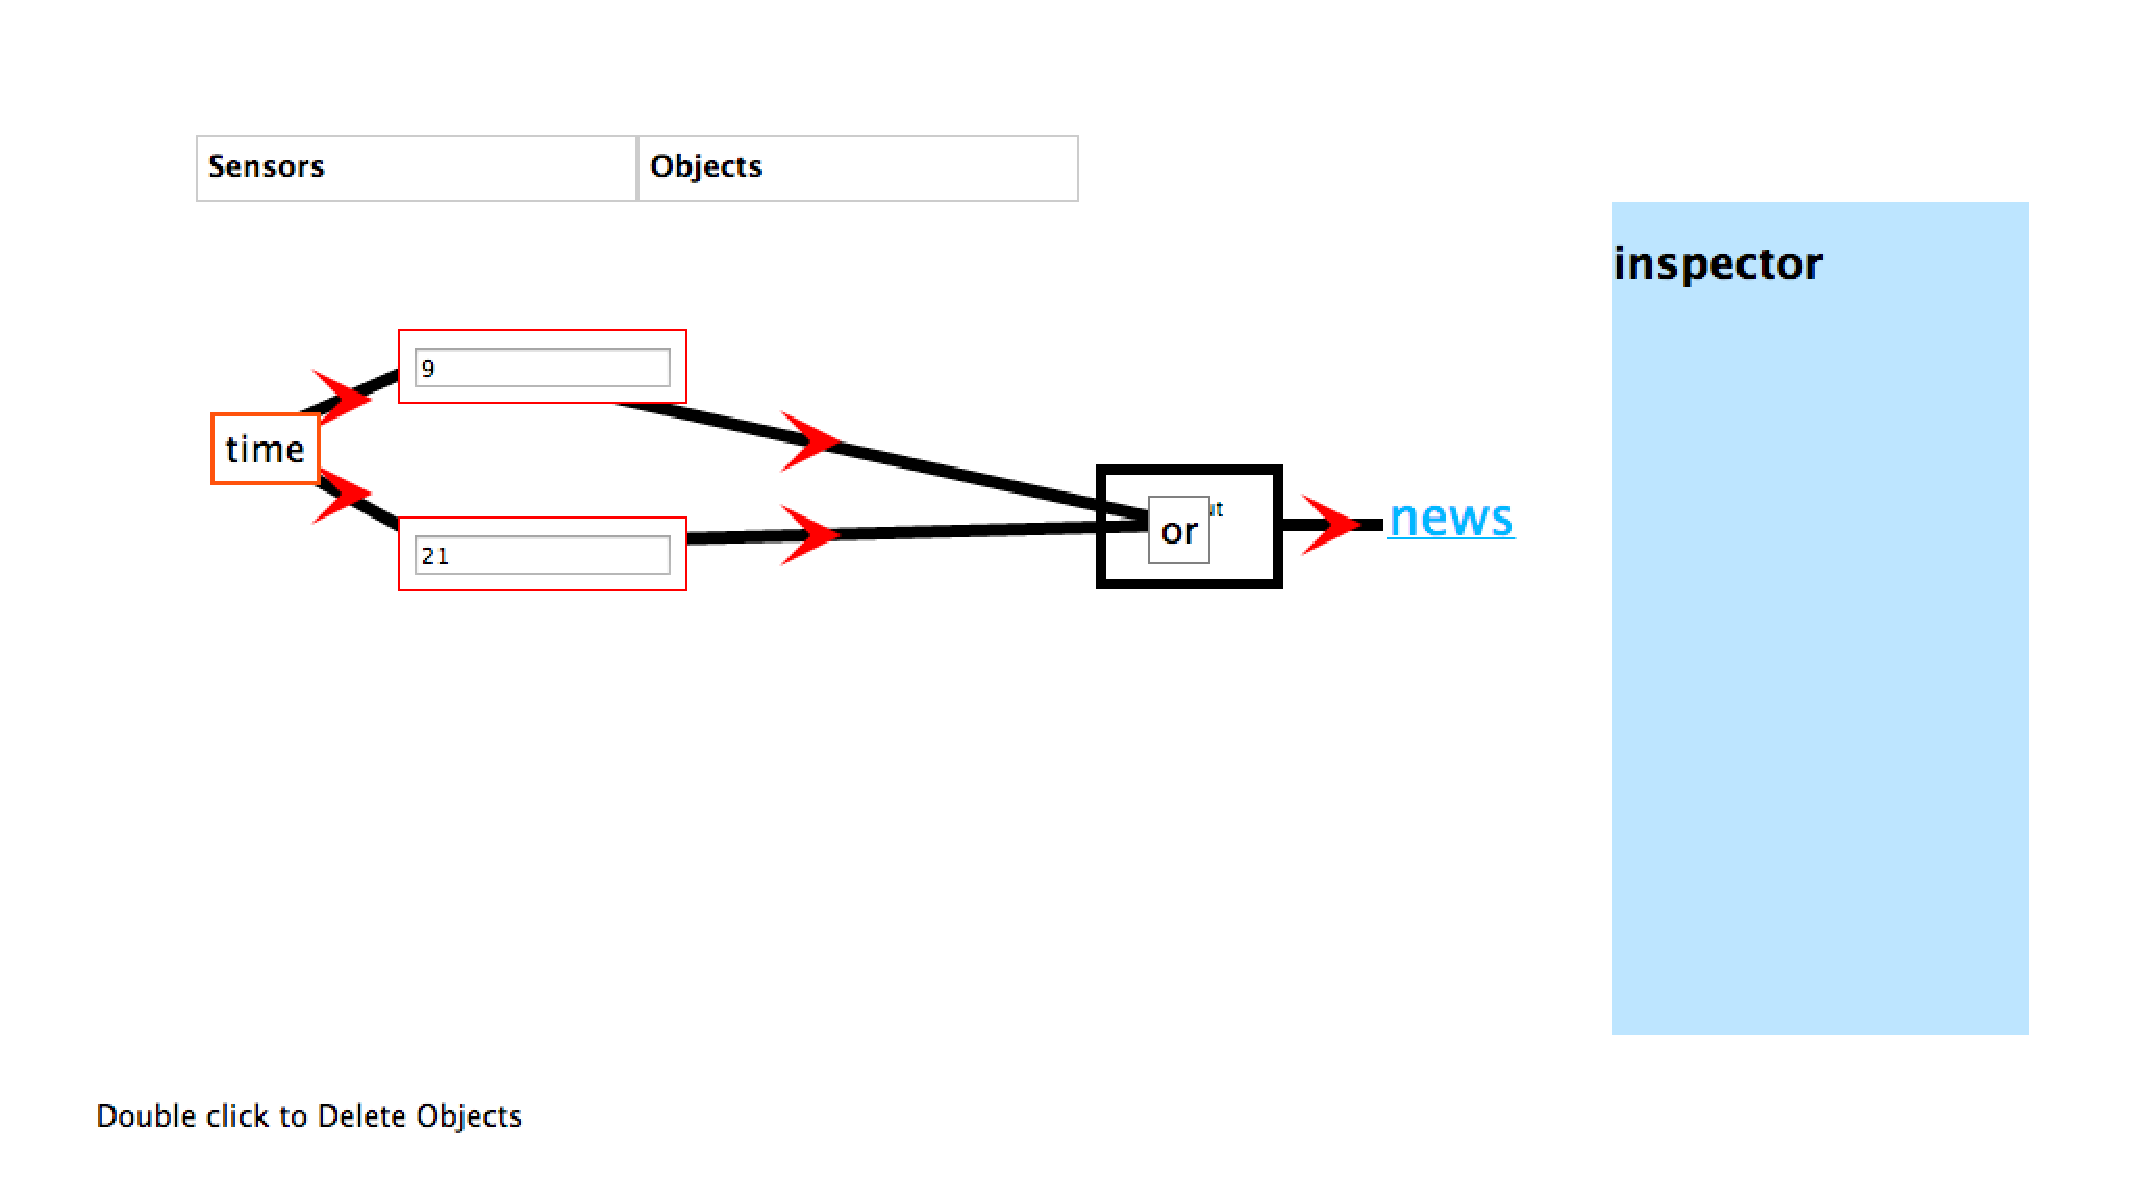
\includegraphics[width=150mm]{image/image10.eps}}
  \end{center}
  \caption{ニュースの購読をビジュアルプログラミング}
  \label{fig:image10}
\end{figure}

\section{超自動ドア}
携帯の位置情報とエレベーターで人があがってきたことをセンシングする。エレベーターがあがってきたという条件と携帯の位置が付近に来たことが送られてくると自動でドアが開く。(図\ref{fig:image14})のようにPOSTリクエストでドアをあける機構を作っておくことで実装可能だ。
(図\ref{fig:image11})はCellPhone\_lonというオブジェクトとCellPhone\_latというオブジェクトがそれぞれ緯度と経度を取得してきている。これをelevatorのデータとマージし、マッチした時にdoorにアクセスしている。
\begin{figure}[htbp]
  \begin{center}
    \fbox{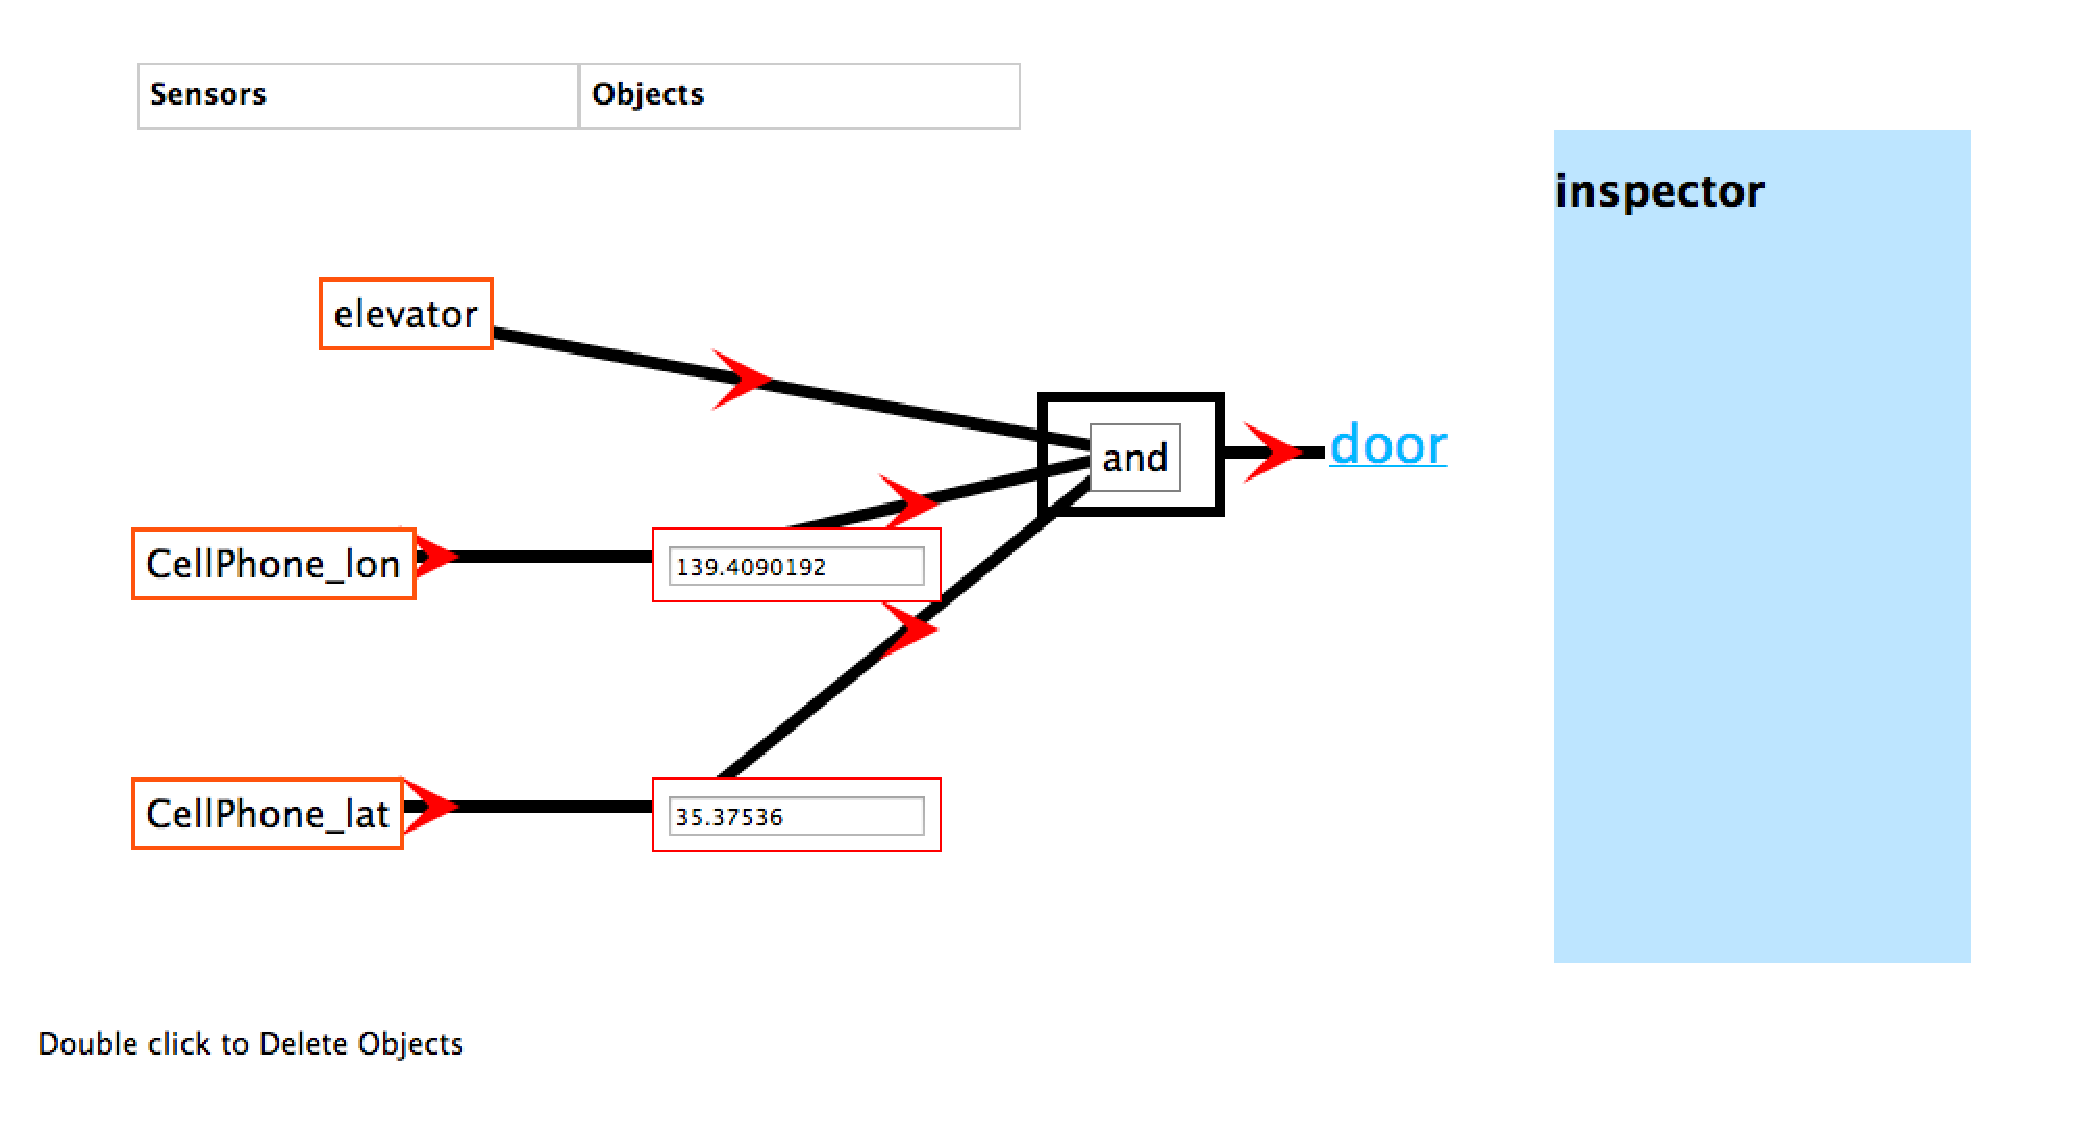
\includegraphics[width=150mm]{image/image11.eps}}
  \end{center}
  \caption{超自動ドアをビジュアルプログラミング}
  \label{fig:image11}
\end{figure}

\begin{figure}[htbp]
  \begin{center}
    \fbox{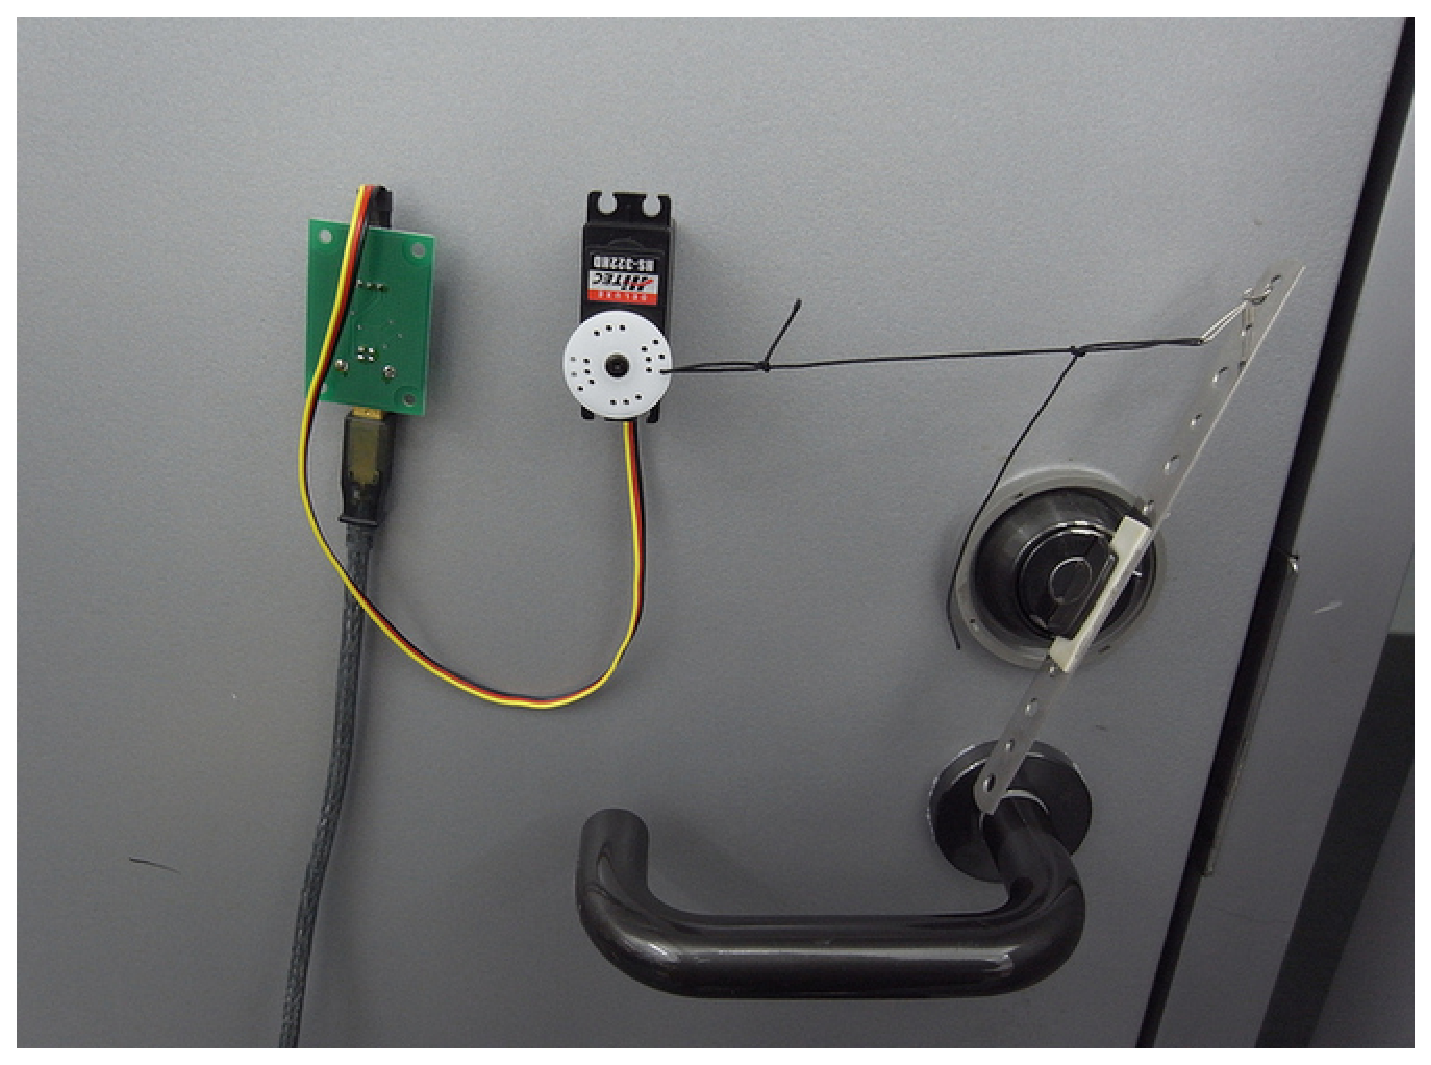
\includegraphics[width=80mm]{image/image14.eps}}
  \end{center}
  \caption{自動解錠するための機構}
  \label{fig:image14}
\end{figure}

\section{忘れ物を通知}
ドアが開いたかどうか、と鞄の中に特定の物があるかというセンシングデータを組み合わせる。ドアが開いた時に鞄の中に物がなかった場合のみ通知をくるように設定し、忘れ物を防止することができる。
(図\ref{fig:image12})のInBagオブジェクトはRFIDタグ\footnote{固有のID情報を埋め込めるタグ}を鞄に設置し、登録した物の有無を検出する。一定時間でtrue/falseを判定し、trueの時だけイベントを発火する。そしてドアが開いた時に鞄の中の財布の有無を確認し、通知することができる。
\begin{figure}[htbp]
  \begin{center}
    \fbox{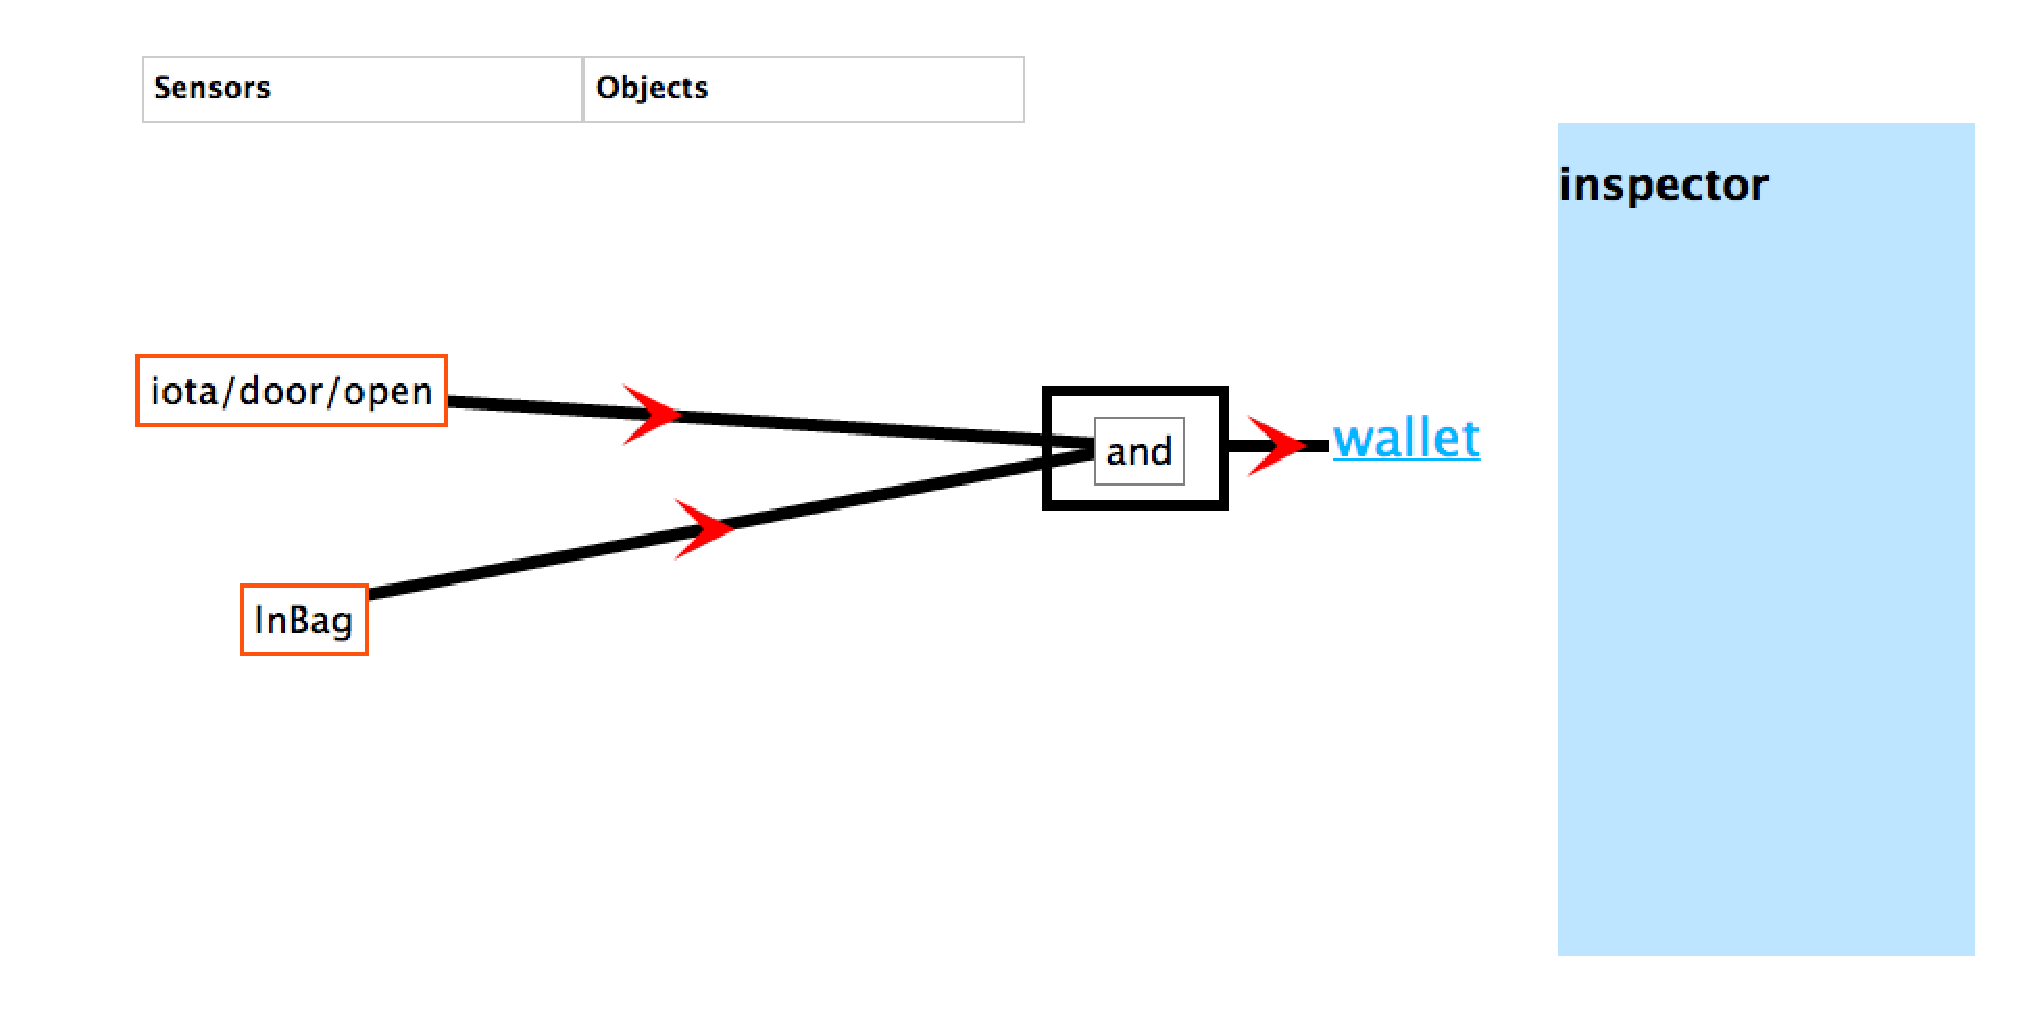
\includegraphics[width=150mm]{image/image12.eps}}
  \end{center}
  \caption{忘れ物検知をビジュアルプログラミング}
  \label{fig:image12}
\end{figure}

\section{カビを通知}
風呂場などに設置するといいだろう。その場所の温度と湿度をセンシングし、カビの発生条件に近いデータにマッチしたらイベントを発火する。また、壁を一定時間ごとに撮影し色の変化を観察することで精度をあげることが出来る。
(図\ref{fig:image13})では温度、湿度、壁の色という3つの要素でカビが発生しそうかどうか判定している。上から、温度20℃から30℃にマッチしたtrue、湿度が80%以上だったらtrue、壁の写真の色平均をとり、RGBの合計が100以下になったら黒ずんできたと判断しtrueとしている。
写真はRaspberry Pi\footnote{http://www.raspberrypi.org/}にWebカメラをつけ、定期的に色平均を計算させている。(図\ref{fig:image15})
\begin{figure}[htbp]
  \begin{center}
    \fbox{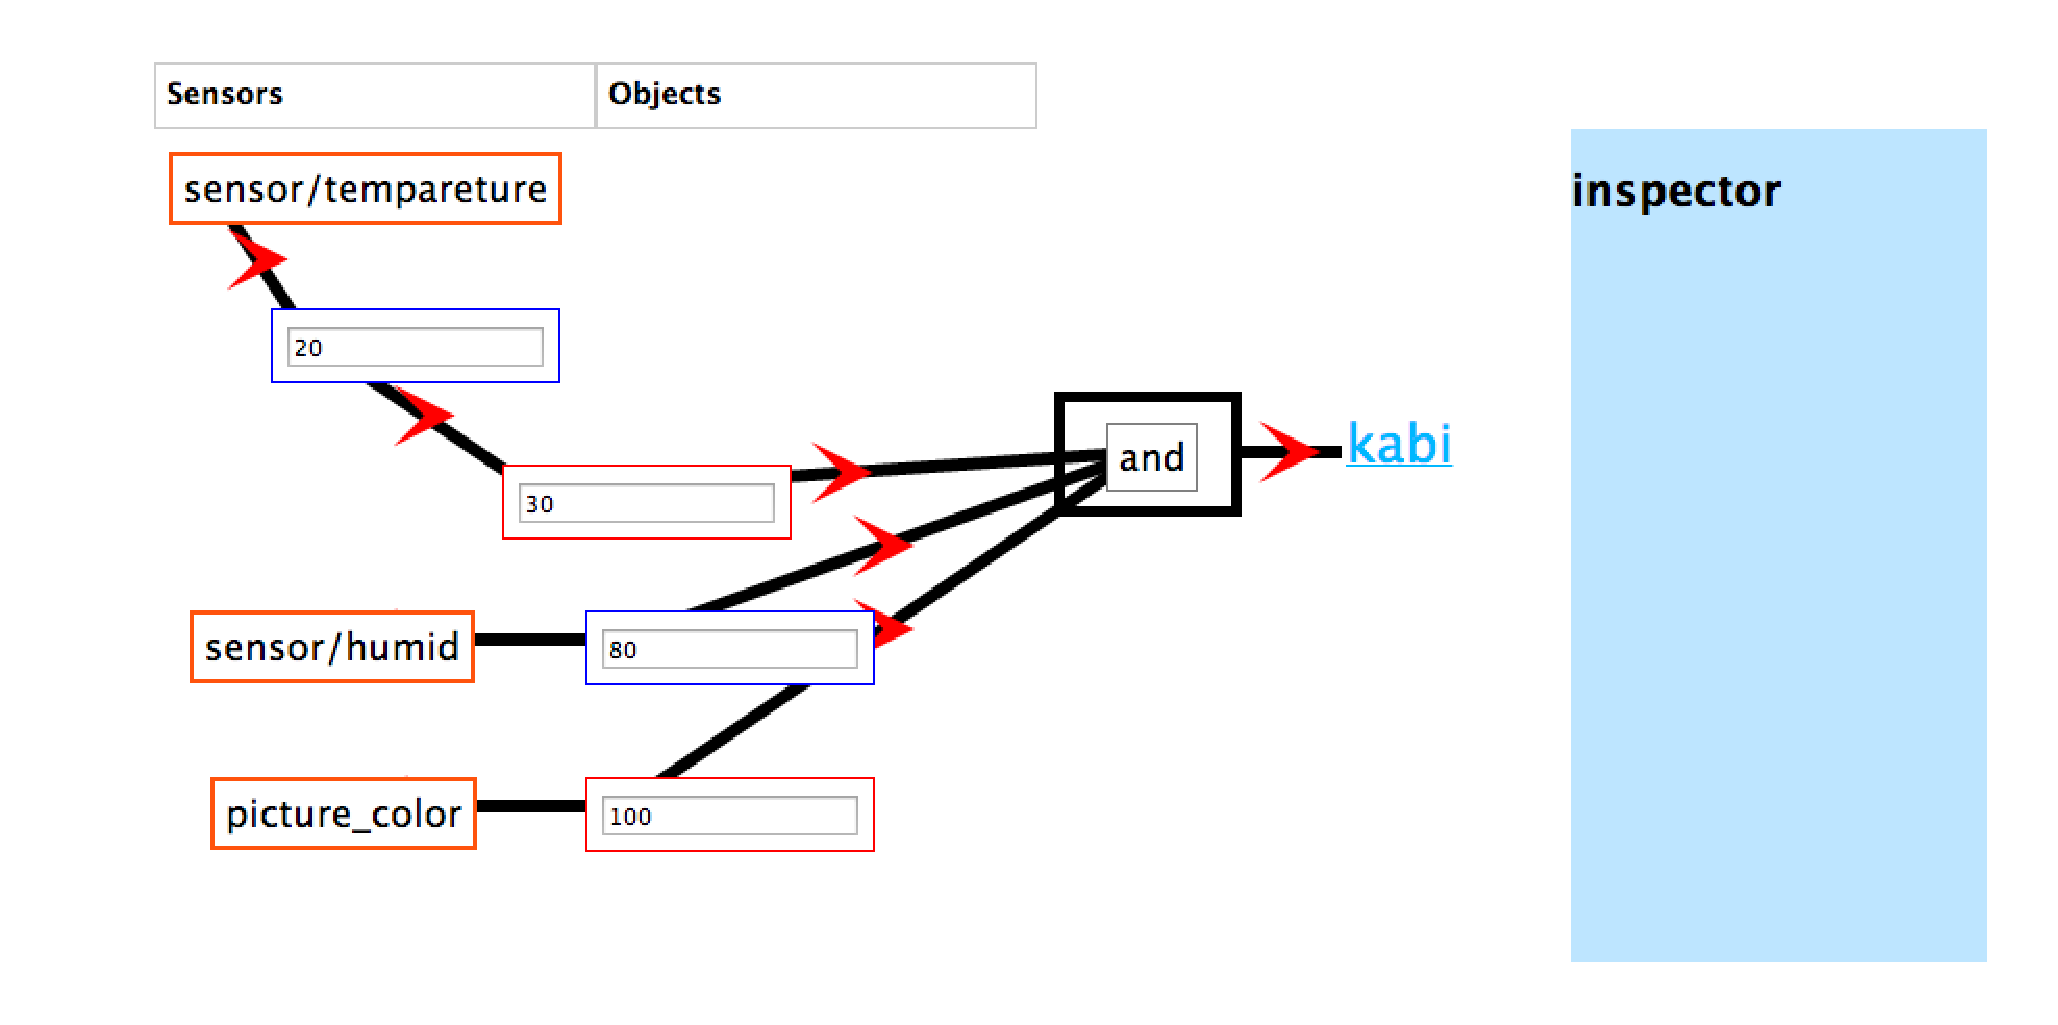
\includegraphics[width=150mm]{image/image13.eps}}
  \end{center}
  \caption{カビの通知をビジュアルプログラミング}
  \label{fig:image13}
\end{figure}

\begin{figure}[htbp]
  \begin{center}
    \fbox{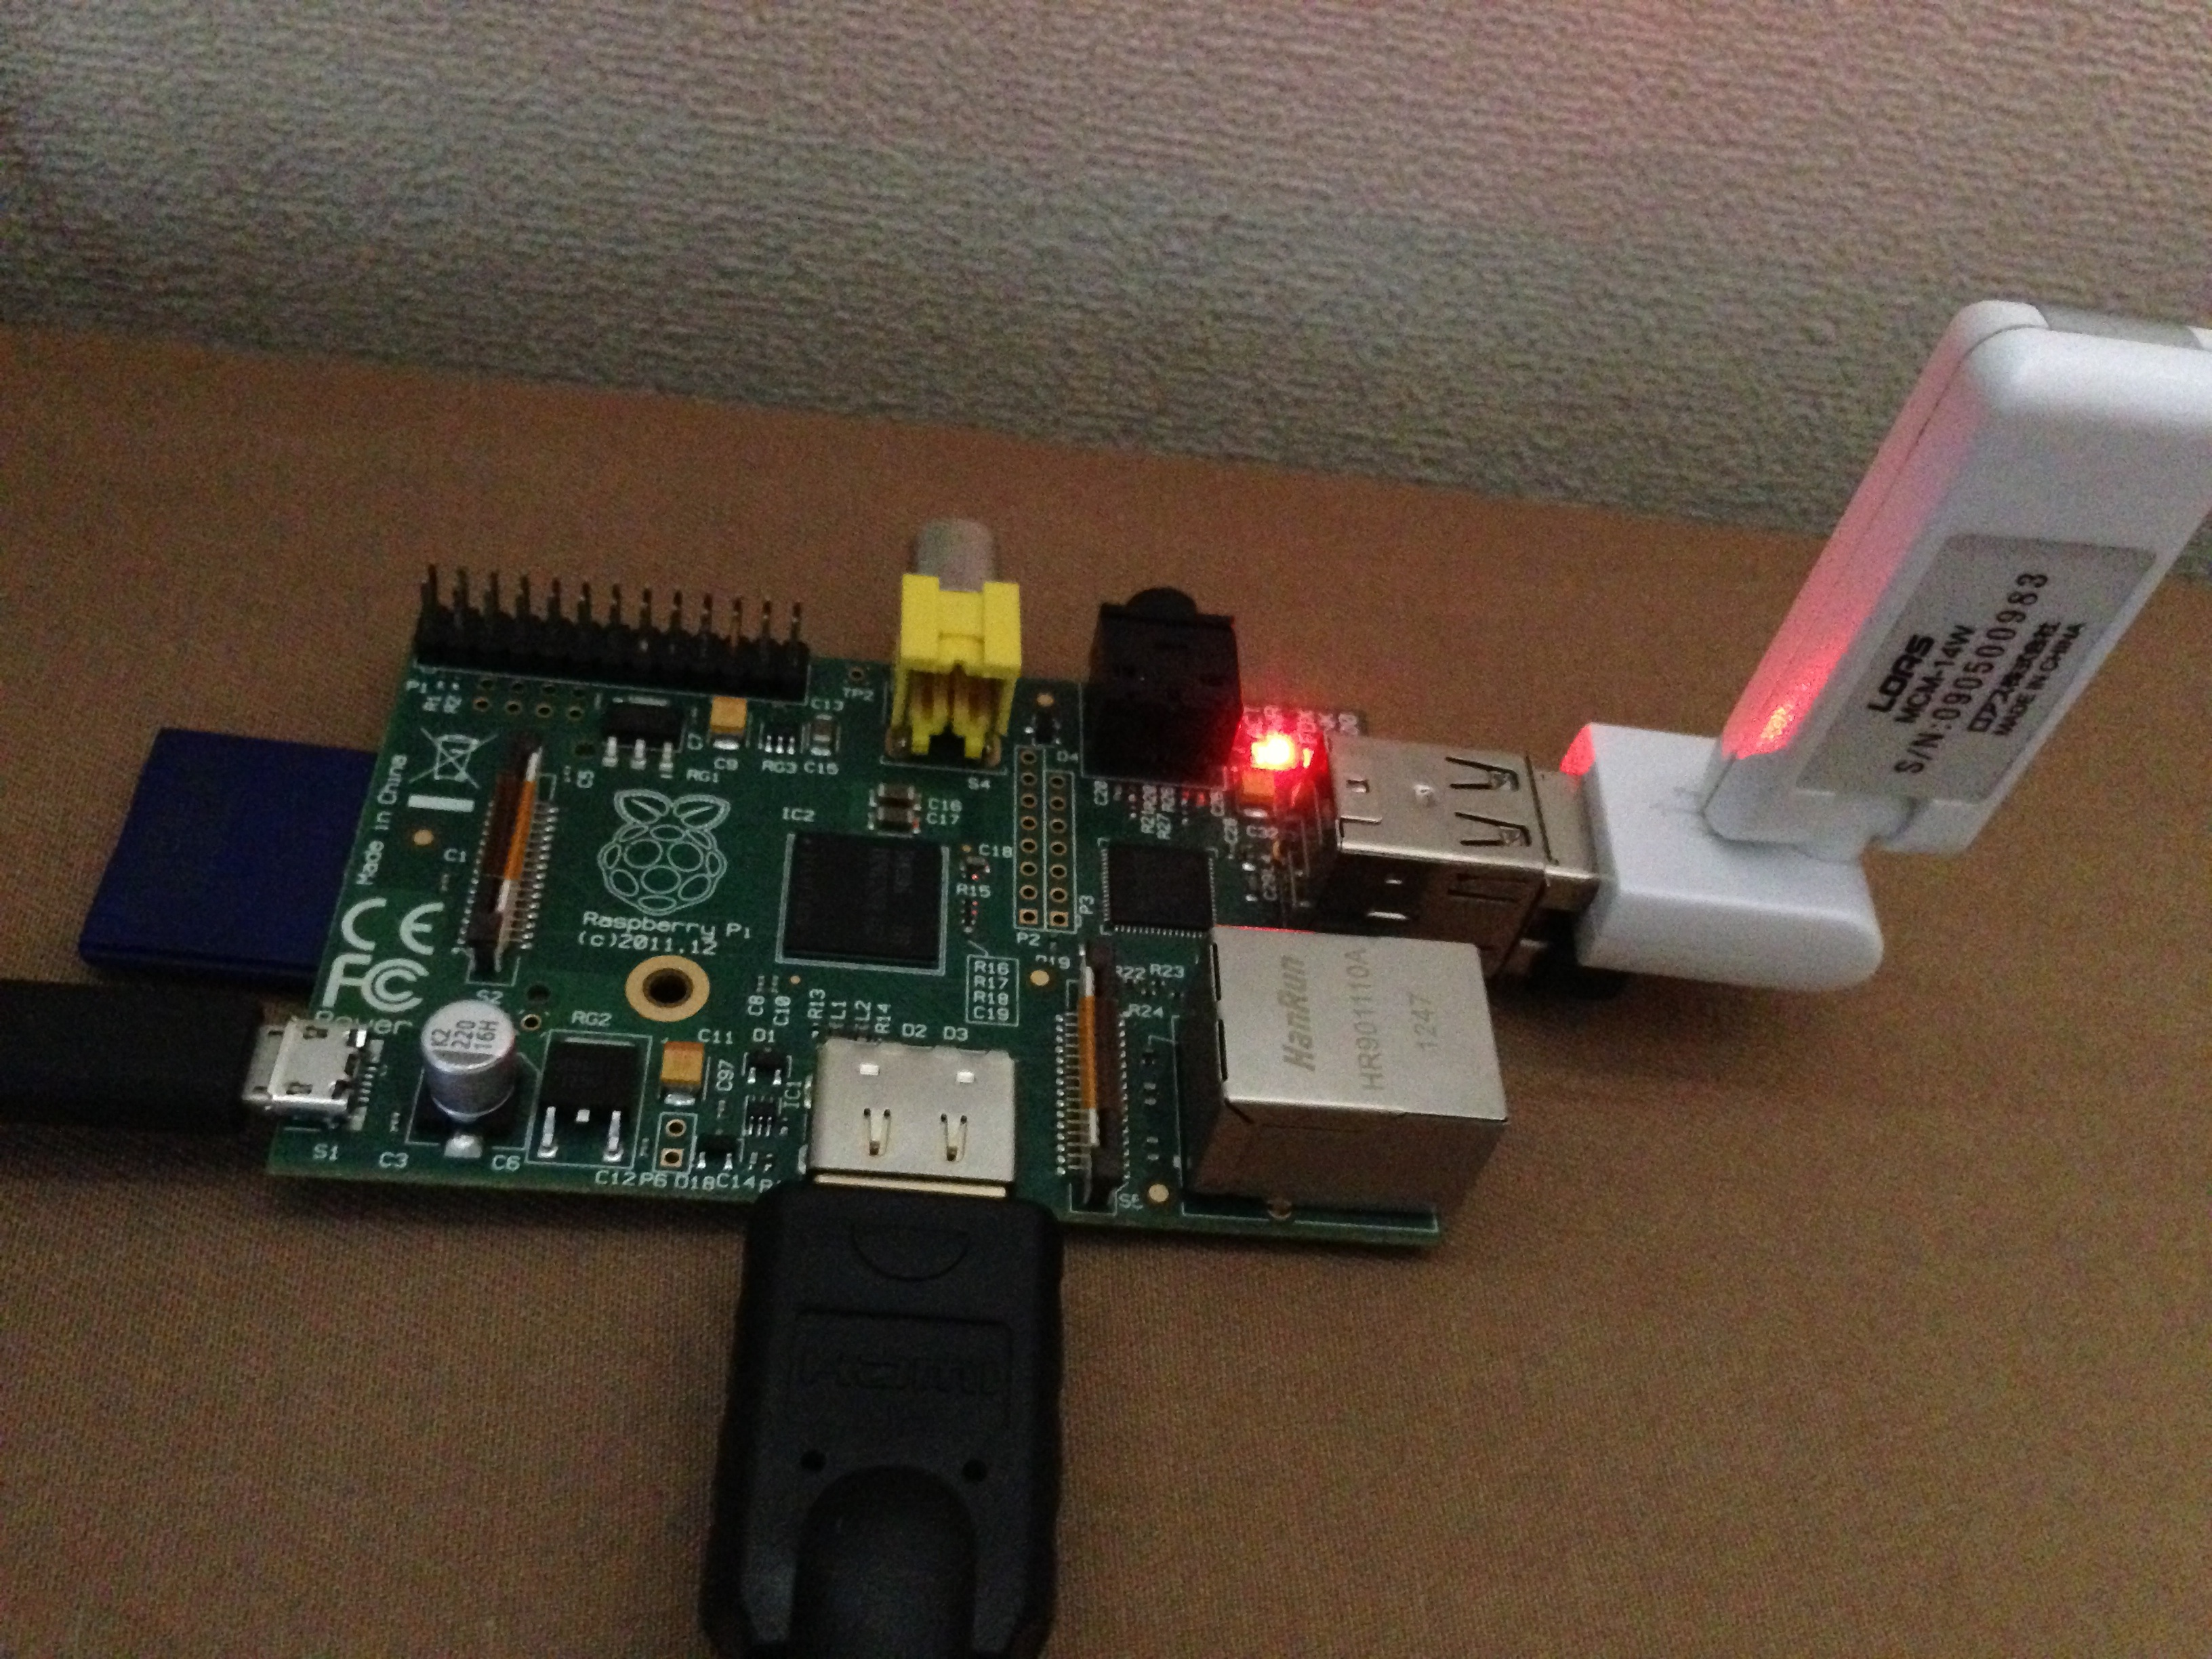
\includegraphics[width=80mm]{image/image15.eps}}
  \end{center}
  \caption{壁の写真をとるための機構}
  \label{fig:image15}
\end{figure}

\section{朝食自動調理}
様々な条件に従って自動で料理を作ってくれるということも簡単にできるだろう。そもそも現状、炊飯器などにタイマーがついていて家電は色々な形で条件指定することができる。Web上で家電を管理することができれば人数や気温、季節、時間など複数の条件分岐を作成すれば複雑な条件で処理させることが可能だろう。
